\documentclass[11pt,a4paper]{article}

% Essential packages
\usepackage[utf8]{inputenc}
\usepackage[T1]{fontenc}
\usepackage[margin=2.5cm]{geometry}
\usepackage{graphicx}
\usepackage{amsmath,amsfonts,amssymb}
\usepackage{booktabs}
\usepackage{hyperref}
\usepackage[font=small,skip=2pt]{caption}  % 
\setlength{\abovecaptionskip}{2pt}  

\graphicspath{{../figures/}}

% Title and author
\title{Test-time Adaptation for Graph-based Molecular Solubility Prediction}
\author{Philipp Sepin\\
        165.164 Selected Topics in Theoretical Chemistry}
\date{\today}

\begin{document}

\maketitle

\begin{abstract}
        Molecular solubility prediction is a critical task in drug development, but models often struggle with distribution shifts between training and test data. This project addresses this challenge by implementing test-time adaptation for graph neural networks and applying it to molecular solubility prediction.

        This project was carried out as part of the seminar 165.164 Selected Topics in Theoretical Chemistry at TU Wien, under the supervision of \href{https://hesther.github.io/}{Prof. Esther Heid}.
\end{abstract}

\section{Introduction}
Molecular solubility prediction is a critical task in drug development, directly impacting a compound's bioavailability and therapeutic potential. Experimental solubility measurement requires substantial time and resources, making computational prediction essential for screening large molecular databases \cite{llompart2024will}.

Recent advances in solubility prediction have been driven by deep learning architectures and molecular embedding approaches. Feature-based neural networks, graph-based neural networks (GNNs), and structural attention methods have emerged as powerful predictive models \cite{llompart2024will}.

However, when there is a distribution shift between the training and test data, as with \textit{AqSolDB} \cite{sorkun2019aqsoldb} and \textit{OChemUnseen} \cite{llompart2024will}, these models often struggle to generalize. This project aims to solve this by utilizing test-time adaptation (TTA) for graph neural networks (GNNs) to shift test set distributions towards the training set distribution, thereby improving generalization.

TTA involves training a model on a source domain, then adapting it at test time by performing a few self-supervised learning (SSL) steps on each test sample before prediction. It has been applied in various domains, such as semantic segmentation, object detection, medical image processing, video depth prediction, question answering, sentiment analysis, entity recognition, speech processing, social network analysis, as well as in protein and enzyme classification \cite{liang2025comprehensive, cui2025online}.

\section{Methods}
\subsection{Dataset}

For this project, the \textit{AqSolDB} dataset \cite{sorkun2019aqsoldb} is used for training and validation. It contains about 8000 molecules as SMILES strings, along with their solubility values. For testing, the \textit{OChemUnseen} dataset \cite{llompart2024will} is used, which contains about 2000 molecules as SMILES strings, along with their solubility values. This dataset is fully orthogonal to the training dataset.

The SMILES strings are converted to molecular graphs using the RDKit library \cite{rdkit2025}, and one-hot encoded node and edge features are added. The node features included element type, number of bonds, electric charge, aromaticity atomic mass, and orbital hybridization, while the edge features included bond order, aromaticity, conjugation, and whether the bond is in a ring. The graphs are then converted to PyTorch Geometric \cite{fey2019fast} data objects.

To enhance the distribution shift, the datasets are filtered as follows:
\begin{itemize}
        \item The training set contains molecules from \textit{AqSolDB} with 6-19 atoms and no amino groups.
        \item The validation set contains molecules from \textit{AqSolDB} with $\leq 5$ atoms and no amino groups.
        \item The first test set (20 Atom set) contains molecules from \textit{OChemUnseen} with $\geq 20$ atoms.
        \item The second test set (NH2 set) contains molecules from \textit{OChemUnseen} with $\geq 20$ atoms and amino groups.
\end{itemize}

\subsection{Model}

The model used for this project is a Y-shaped architecture, consisting of a shared encoder, which branches into a decoder and a prediction head, as shown in Figure \ref{fig:model}.

\begin{figure}[htbp]
        \centering
        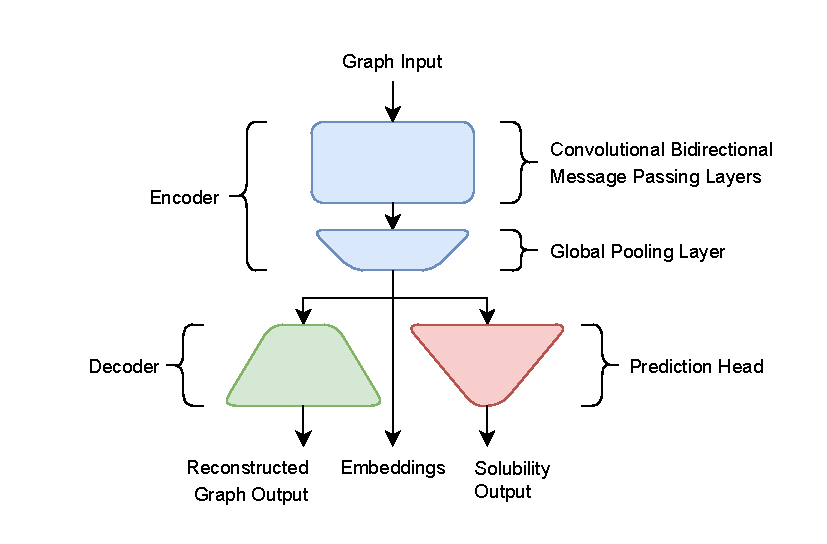
\includegraphics[width=1\textwidth]{model.pdf}
        \caption{The model architecture.}
        \label{fig:model}
\end{figure}

The encoder is a convolutional bidirectional message passing neural network (MPNN), a GNN that applies convolutional operations to aggregate information from neighboring nodes in both directions through iterative message passing. It consists of two graph convolutional layers which return an embedding vector of size 16 for each node. These nodal embedding vectors are an information-dense representation of the molecular graph. A 2D projection of the mean-pooled 16-dimensional embedding space with corresponding solubility values is shown in Figure \ref{fig:solubility}, visualized using two dimensionality reduction techniques, t-SNE \cite{van2008visualizing} and UMAP \cite{mcinnes2018umap}.

The decoder consists of two fully connected layers that reconstruct node and edge features from the nodal embedding vectors. The prediction head employs a global pooling layer which aggregates the nodal embedding vectors into a single global embedding vector by taking their mean, followed by two fully connected layers that map the global embedding vector to the predicted solubility value, creating a multi-task learning architecture.

\begin{figure}[htbp]
        \centering
        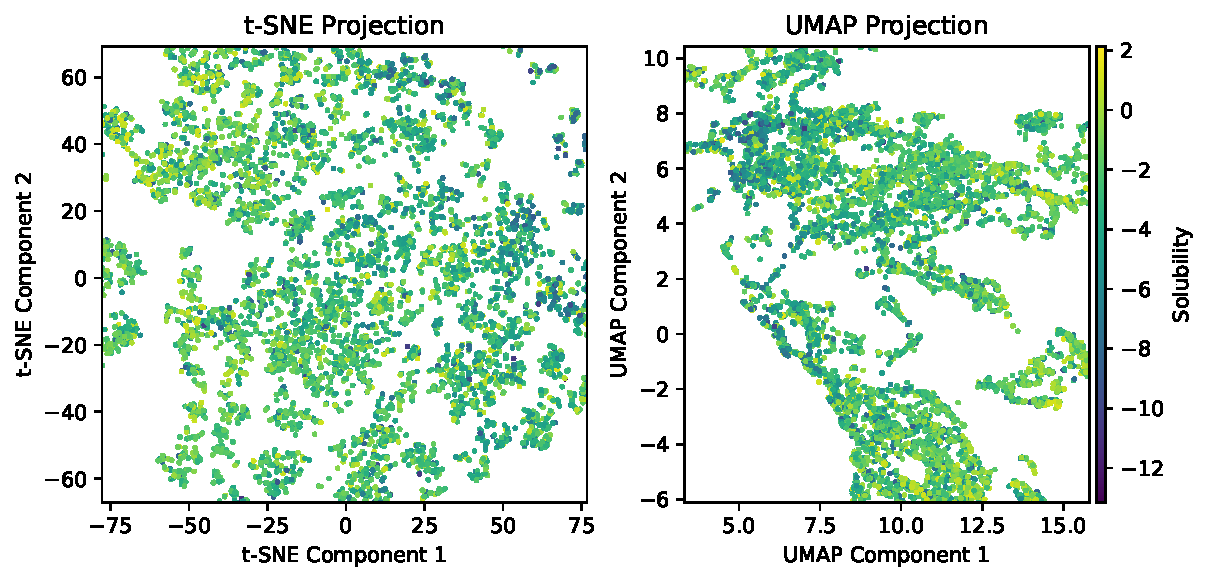
\includegraphics[width=1\textwidth]{solubility.pdf}
        \caption{2D projection of the embedding vectors with their corresponding solubility.}
        \label{fig:solubility}
\end{figure}

\subsection{Training}

Following our architecture design, the model can be trained on two tasks. The first one is a self-supervised task, where masked node and edge features are denoised and reconstructed. For this, all features of a certain percentage of nodes and edges are masked. The encoder then learns to create an information-dense representation in form of the nodal embedding vectors, from which the decoder learns to reconstruct the denoised node and edge features. The second task is the supervised task, where the encoder also learns to create nodal embedding vectors, from which the prediction head learns to predict the solubility value.

Following the literature, both tasks are trained simultaneously by combining their respective losses \cite{cui2025online, wang2022test}. We implemented this by summing the weighted denoising and prediction losses, weighting the denoising loss twice as high as the prediction loss.

The model was trained for 70 epochs with a batch size of 1024 using the Adam optimizer. Hyperparameters were optimized on the validation set. The learning rate was optimized to $5 \cdot 10^{-3}$ and training was performed on a single NVIDIA GeForce GTX 960M GPU.

\begin{figure}[htbp]
        \centering
        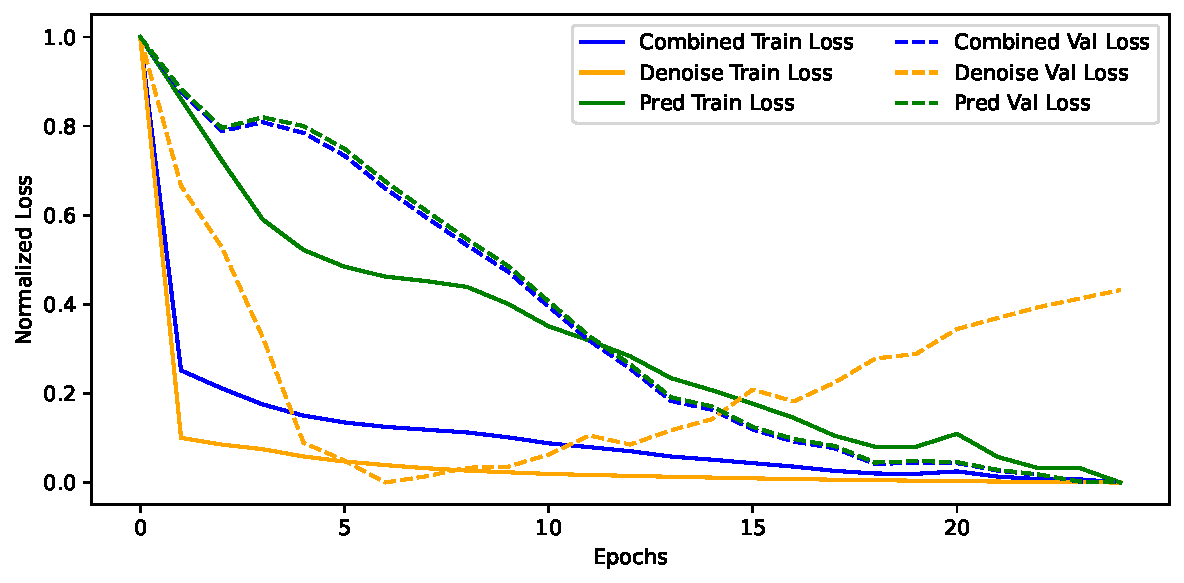
\includegraphics[width=1\textwidth]{loss_plot.pdf}
        \caption{Training and validation losses.}
        \label{fig:loss_plot}
\end{figure}

As shown in Figure \ref{fig:loss_plot}, the denoising validation loss steadily decreases, whereas the prediction validation loss showed an interesting double-descent behaviour, where it first converges at around 10 epochs, then increases again, and finally converges at around 60 epochs.

\subsection{Test-time Adaptation and Prediction}

For TTA, each test sample is processed individually. The encoder is adapted to the specific molecular structure through a few gradient descent steps on the self-supervised loss, after which the adapted model predicts the solubility using the standard prediction head. The model is then reset to its original state for the next test sample. The step size and number of gradient steps were optimized to $1.9 \cdot 10^{-3}$ and 5 steps, respectively.

The distribution shift and effect of TTA can be seen in the 2D projections of the embedding space shown in Figures \ref{fig:sets} and \ref{fig:sets_TTA}.

\begin{figure}[htbp]
        \centering
        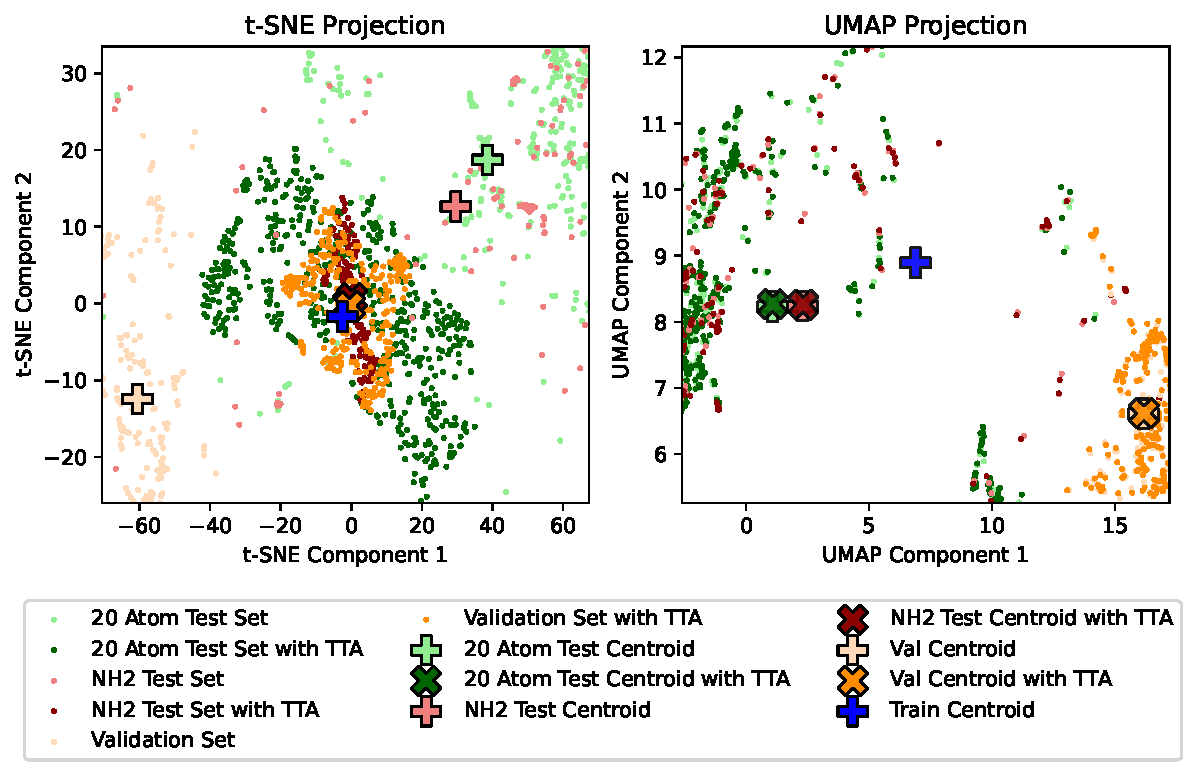
\includegraphics[width=1\textwidth]{sets_TTA.pdf}
        \caption{2D projection of the embedding vectors before and after TTA.}
        \label{fig:sets_TTA}
\end{figure}

\section{Results}

\begin{table}[htbp]
        \centering
        \begin{tabular}{@{}lccc@{}}
                \toprule
                \textbf{Model}    & \textbf{Validation RMSE} & \textbf{Test RMSE (20 Atom set)} & \textbf{Test RMSE (NH2 set)} \\
                \midrule
                Model without TTA & 1.3886                   & 1.8705                           & 1.8898                       \\
                Model with TTA    & 1.2675                   & 2.0093                           & 2.1690                       \\
                Reference Model   & 1.2540                   & 2.2291                           & 2.1379                       \\
                \bottomrule
        \end{tabular}
        \caption{Performance comparison of different model configurations.}
        \label{tab:results}
\end{table}

As shown in Table \ref{tab:results}, TTA worsened performance on both test sets, but improved validation performance. Figure \ref{fig:sets_TTA} shows that TTA shifted the test and validation set embeddings. The t-SNE projection shows a clear shift towards the training set distribution, whereas the UMAP projection shows shifts in other directions, which aligns with the observed performance degradation. This suggests that UMAP, with its focus on preserving global structure, may be more suitable for analyzing the effects of TTA.

A reference model trained only on the prediction task shows that SSL training can help generalization, as the reference model had worse performance on both test sets, but slightly better validation performance.

Additional figures are provided in the appendix. The code for this project is available at \href{https://github.com/p0017/Molecular-Test-Time-Adaptation}{github.com/p0017/Molecular-Test-Time-Adaptation} under the \href{https://www.gnu.org/licenses/gpl-3.0}{GPL-3.0} license.

\section{Conclusion}

This study implemented test-time adaptation (TTA) for graph neural networks (GNNs) and applied it to molecular solubility prediction. While TTA successfully shifted the distributions of the validation and test sets, the shift did not consistently move them closer to the training set distribution, resulting in partially worse predictive performance. Future work could explore alternative self-supervised learning (SSL) tasks, different adaptation strategies, or investigate TTA effectiveness on datasets with different distribution shifts.

\bibliographystyle{plain}
\bibliography{references}

\section{Appendix}

\begin{figure}[htbp]
        \centering
        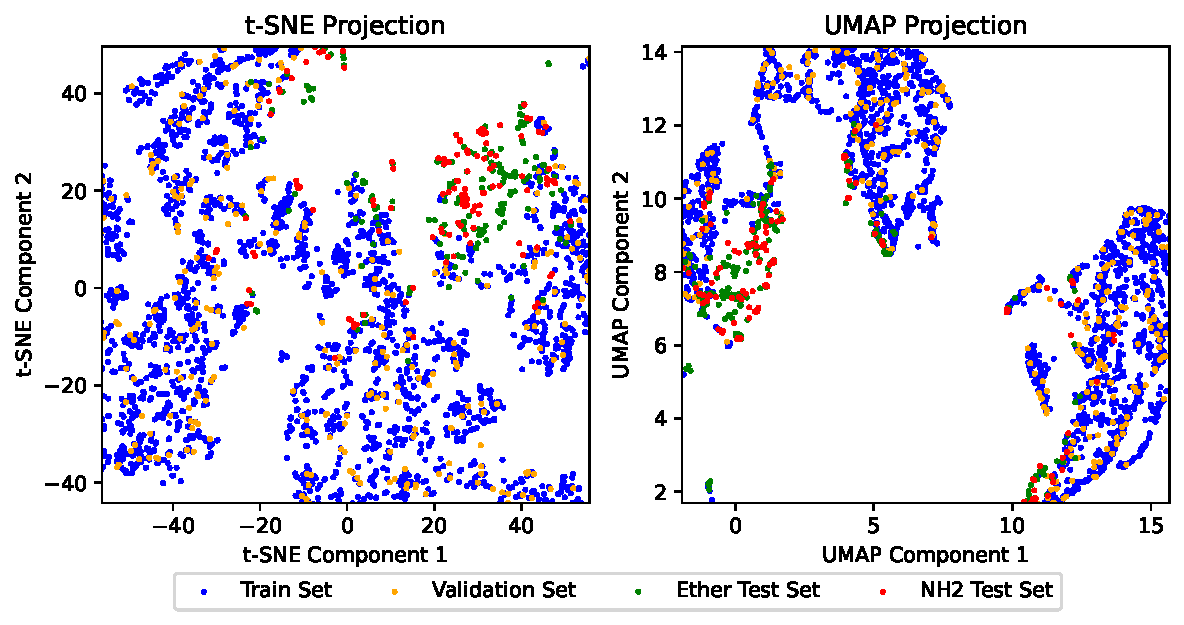
\includegraphics[width=1\textwidth]{sets.pdf}
        \caption{2D projection of the embedding vectors with their corresponding sets.}
        \label{fig:sets}
\end{figure}

\begin{figure}[htbp]
        \centering
        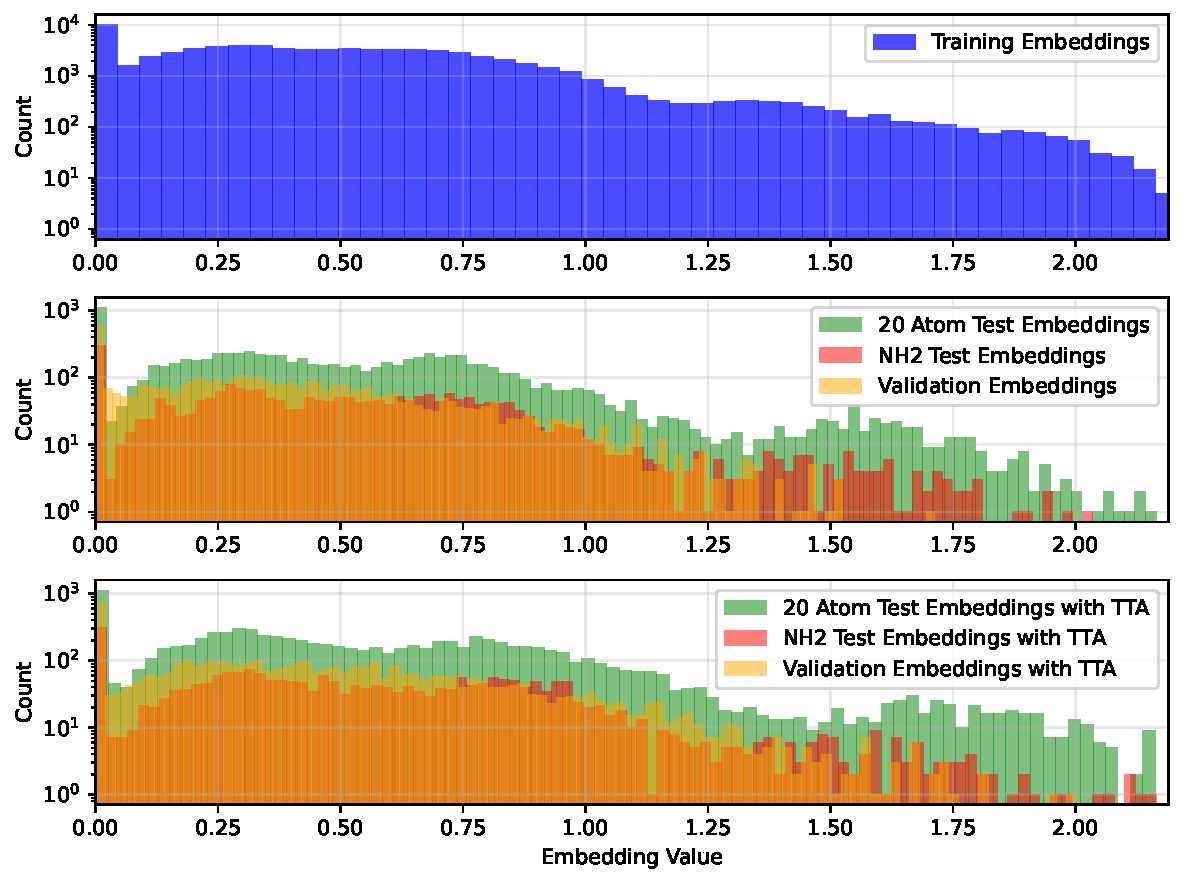
\includegraphics[width=1\textwidth]{embedding_histogram.pdf}
        \caption{Histogram of the embedding vector components.}
        \label{fig:embedding_histogram}
\end{figure}

\begin{figure}[htbp]
        \centering
        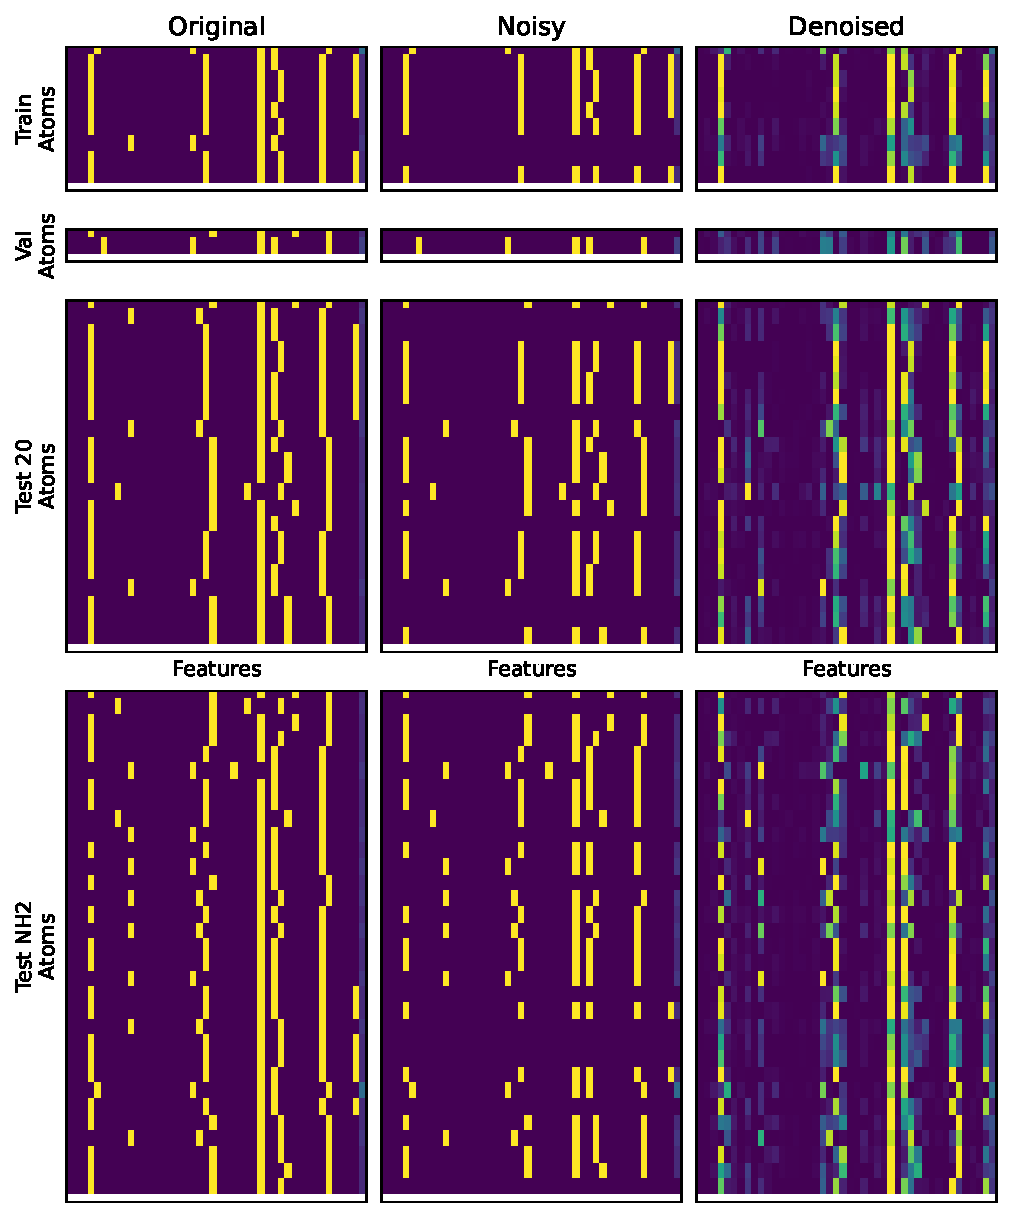
\includegraphics[width=1\textwidth]{feature_visualization_node.pdf}
        \caption{Original, masked, and reconstructed node features.}
        \label{fig:feature_visualization_node}
\end{figure}

\begin{figure}[htbp]
        \centering
        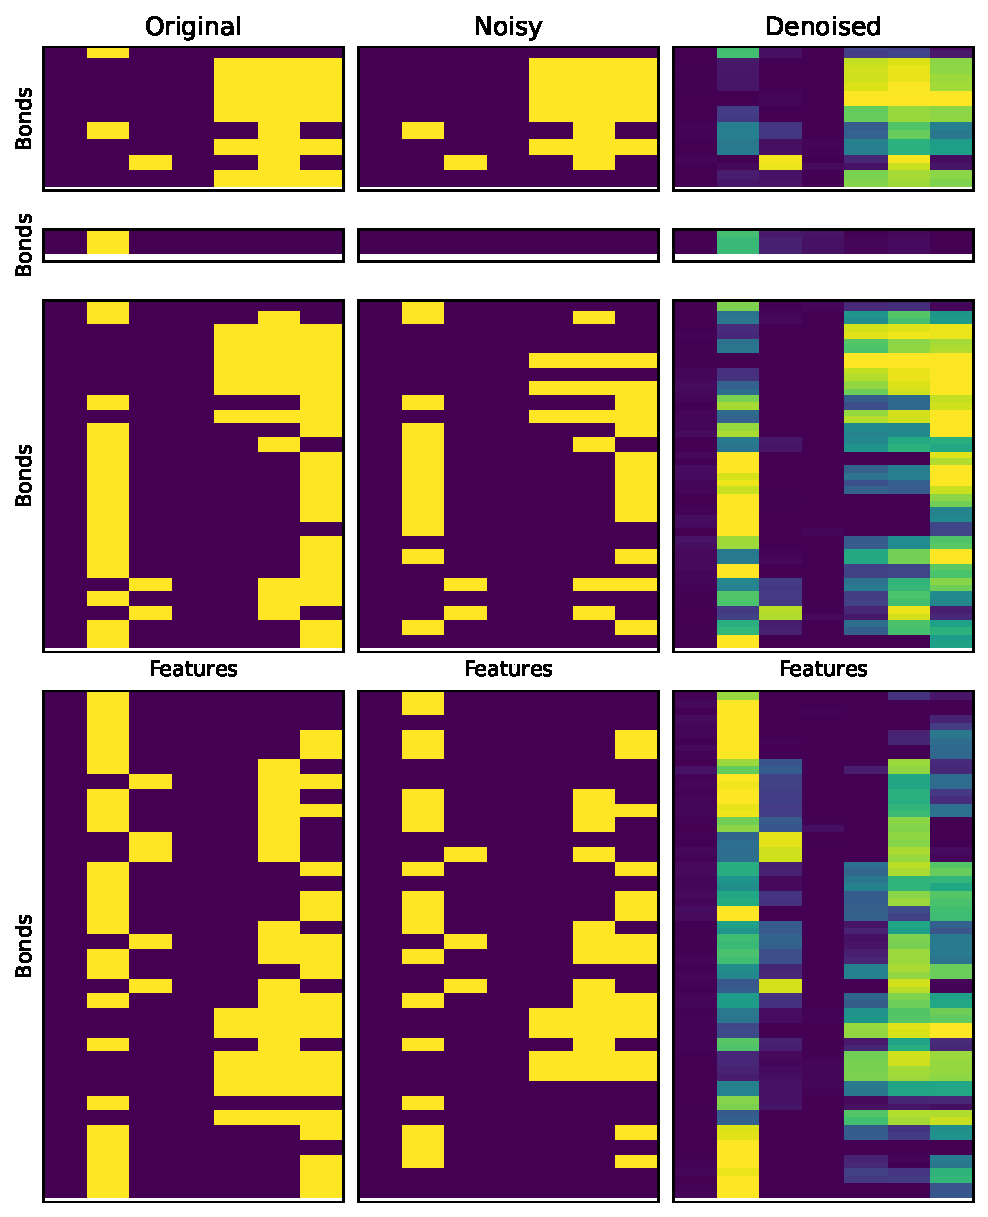
\includegraphics[width=1\textwidth]{feature_visualization_edge.pdf}
        \caption{Original, masked, and reconstructed edge features.}
        \label{fig:feature_visualization_edge}
\end{figure}

\end{document}